\documentclass[man,bazy,a4paper,11pt,sfheadings,noindentfirst]{mgrwms}
\usepackage[utf8]{inputenc}
\usepackage[T1]{fontenc}
\usepackage{polski}
\usepackage{amsfonts}
\usepackage{amsmath}
\usepackage{amssymb}
\usepackage{amsthm}
\usepackage{geometry}
\usepackage{clrscode}
\usepackage{lmodern}
\usepackage{tocloft}
\usepackage{graphicx}
\usepackage{hyperref}
\usepackage{setspace}
\hypersetup{%
	pdfauthor={Michał Nowak},%
	pdftitle={Zarządzanie jakością usług dla pamięci dyskowych},%
	pdfborder={0 0 0},%
	pdfkeywords={},%
	pdfstartview=FitH,%
	hypertexnames=false%
}
\usepackage{mastersthesis}
\usepackage{algorithmic,algorithm}
\makeatletter
\renewcommand{\ALG@name}{Algorytm}
\renewcommand{\listalgorithmname}{Lista \ALG@name ów}
\makeatother

\begin{document}

\title{Zarządzanie jakością usług dla pamięci dyskowych}
\author{Michał Nowak}
\promotor{dr inż.\ Darin Nikolow}
\nralbumu{228971}
\keywords{quality of service, linux, fuse, vfs, file systems, disk storage, \FPclass, \sharpPclass-complete}

\maketitle

\renewcommand{\cfttoctitlefont}{\LARGE\sffamily\bfseries}
\renewcommand{\cftchapfont}{\sffamily\bfseries}
\renewcommand{\cftchappagefont}{\sffamily\bfseries}
\renewcommand{\cftsecfont}{\sffamily}
\renewcommand{\cftsecleader}{\sffamily\cftdotfill{\cftsecdotsep}}
\renewcommand{\cftsecpagefont}{\sffamily}
\setlength{\cftbeforechapskip}{3.75mm}

\tableofcontents

\vskip1in

\chapter{Wstęp} \label{ch:introduction}

\section{Problem}

Celem tej pracy jest stworzenie systemu plików z mechanizmem
\textbf{Quality of Service (QoS)}, który będzie kształtował i ograniczał przepustowość dysku oraz pozwoli na zapewnienie sprawiedliwego względgem szybkości
dostępu do zasobów dyskowych.

\section{Cel badawczy}

Praca niniejsza ma na celu implementację mechanizmu \textbf{QoS} w systemie przechowywania danych,
pozwalającej na kontrolowanie szybkości transferu danych odczytu i zapisu operacji I/O.

Tego typu system taki mógłby być przydatny np. w strumieniowaniu dużych plików multimedialnych dla wielu klientów.
Zapewnienie minimalnej szybkości transferu danych podczas odczytu plików może znacząco podnieść wydajność
takich usług.

\subsection{Cel praktyczny}
Zaimplementowany zostanie system plików o nazwie \textbf{QoSFS}\footnote{Quality of Service Filesystem}, który pozwoli na ustalanie minimalnej potrzebnej szybkości transferu danych do wykonywania operacji I/O.

\subsection{Cel teoretyczny}
Teoretyczna część pracy zawiera analizę wykonanego systemu pod kątem przydatności,
opóźnień odczytu i zapisu oraz ewentualnych przeciążeń w komunikacji.
W tym celu stworzone zostana odpowiednie benchmarki wykonujące operacje na plikach,
które umożliwiają analizę zaimplementowanego rozwiązania.

\section{Struktura pracy}

\begin{itemize}
  \item Rozdział \textbf{\ref{ch:introduction}}
	opisuje postawione cele - teoretyczny i praktyczny oraz zawiera opis struktury pracy.

	\item W rozdziale \textbf{\ref{ch:subject-introduction}} znajduje się
	wprowadzenie do tematyki pracy oraz opis wykorzystanych technologii. 
	Wytłumaczono jak działa wirtualny system plików, opisano
    ideę systemu plików w przestrzeni użytkownika i wybraną metodę
    testowania zaimplementowanego rozwiązania.

	\item Rozdział \textbf{\ref{ch:articles}} przeznaczony jest na przegląd
    artykułów, które zostały wykorzystane podczas pracy.
    
    \item W rozdziale \textbf{\ref{ch:prototypes}} opisano wszystkie rozważane rozwiązania,
    które nie znalazły się w pracy oraz wytłumaczono powody, dla których
    z nich zrezygnowano.
    
    \item Projekt oraz implementacja systemu zostały przedstawione w rozdziale \textbf{\ref{ch:implementation}}.
    Znajduje się tam projekt modelu systemu oraz dokładny opis każdego
    z modułów oraz sposobu ich testowania.
    
    Dodatkowo można tam znaleźć instrukcję użytkownika (instalacja i uruchomienie systemu)
    oraz narzędzia użyte podczas procesu implementacji.
    
    \item W rozdziale \textbf{\ref{ch:experiments}} scharakteryzowano
    system, na którym przeprowadzono testy i przedstawiono wyniki
    oraz ich analizę.
    
    \item Ostatni rozdział \textbf{\ref{ch:summary}} poświęcony jest na
	wnioski oraz prezentację możliwych kierunków rozwoju systemu.
    
    \item W końcowej części pracy znajduje się bibliografia.
\end{itemize}

\chapter{Wprowadzenie do tematyki} \label{ch:subject-introduction}

Aby sprostać wymaganiom stawianym przez rozwój technologiczny, systemy przechowywania
danych z roku na rok stają się coraz pojemniejsze i szybsze. W porównaniu z pierwszym dyskiem twardym, który mógł przechowywać zaledwie 5MB danych, aktualna standardowa pojemność dysków jest
mniej wiecej 200,000 razy wieksza.

\begin{figure}[h!]
	\centering
	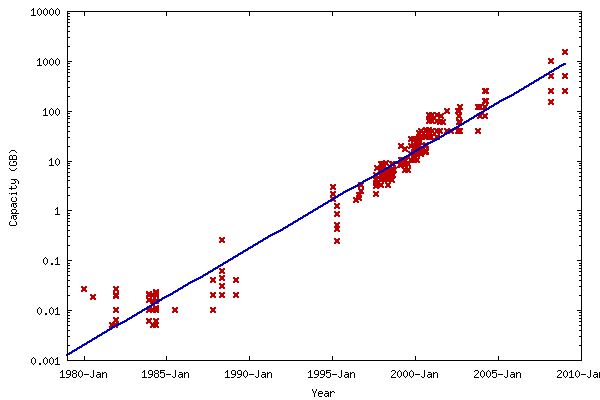
\includegraphics[scale=0.5]{HDDOverTime.png}
		\caption{Zmiana pojemności dysków na przestrzeni lat}
\end{figure}

Ponadto, przechowywane dane należą do różnych typów, z których wiele może mieć narzucone pewne wymagania
szybkości transferu danych. Na przykład, gdy otwieranie dużego pliku tekstowego zajmuje kilka lub
kilkanaście minut, nie jest to tak uciążliwe jak kilkusekundowe wczytywanie każdej klatki
pliku multimedialnego.

Quality of Service jest używany głównie w telekomunikacji, gdzie administratorzy
sieci mogą go używać do zapewnienia przepustowości dla krytycznych aplikacji aby ich transakcje zostały przetworzone w akceptowalnym czasie.

\section{Virtual File System}
System będzie działać w oparciu o
\textbf{VFS (Virtual File System)} w systemie Linux. VFS jest abstrakcyjną powłoką
leżącą ponad rzeczywistym systemem plików. Jej zadaniem jest umożliwienie procesom korzystania z niego w jednakowy sposób niezależnie od
aktualnie używanego systemu plików. Architekturę  VFS przedstawiono na rysunku \ref{fig:vfs}.

\begin{figure}[h!]
	\centering
	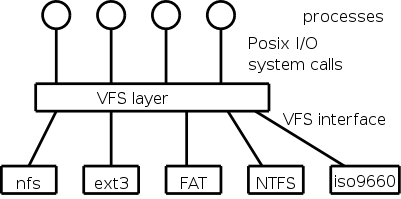
\includegraphics[scale=0.5]{vfs.png}
	\caption{Architektura Virtual File System}
    \label{fig:vfs}
\end{figure}

\section{File System in Userspace}
Do stworzenia QoSFS użyty zostanie moduł jądra, który umożliwia programowanie
logiki systemu plików - \textbf{FUSE (Filesystem in USErspace)}. 

\begin{figure}[h!]
	\centering
	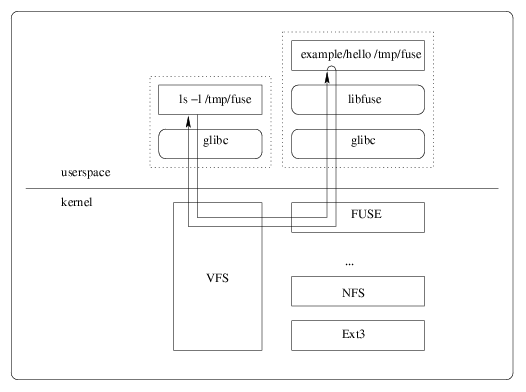
\includegraphics[scale=0.5]{fuse_structure.png}
		\caption{Struktura FUSE}
        \label{fig:fuse}
\end{figure}

Jest on szeroko znany i często używany
oraz stanowi bazę popularnego w GNU/Linux sterownika ntfs-3g\footnote{umożliwia
on dostęp odczytu/zapisu do systemu NTFS}.

Struktura FUSE przedstawiona została na rysunku \ref{fig:fuse}.

FUSE pozwala na programowanie w przestrzeni użytkownika, oraz konfigurację poprzez
pliki i aktualizację wersji bez restartu. 
Dzięki dostępowi do przestrzeni użytkownika będzie możliwe wykorzystanie standardowych
bibliotek bibliotek C.

\section{Flexible I/O tester}
Do testowania przepustowości użyte zostanie narzędzie \textbf{fio (flexible I/O tester)}.

Fio jest benchmarkiem wydajności I/O w systemach Unix, który pozwoli na
ocenienie poprawności zaproponowanego rozwiązania.

\chapter{Przegląd artykułów} \label{ch:articles}
W poniższym rodziale przedstawiono artukuły, które wykorzystane zostały
podczas pracy nad systemem.

\section{Providing Quality of Service in Object-Based File System}

Artykuł autorstwa Joela C. Wu, Scotta A. Brandta, powstał na \textit{University of California} w Santa Cruz.
Opisuje on framework \textbf{Bourbon}, który został zaprojektowany do pracy
z rozproszonym obiektowym systemem przechowywania danych \textbf{Ceph}\footnote{http://ceph.com/ceph-storage/file-system/}

Bourbon działa na podstawie wartości wagowych. Dzieli maksymalną przepustowość dysku
pomiędzy procesy i nadaje im maksymalną szybkość transferu danych bazując na 
nadanych wagach. Jeżeli proces A posiada wagę \texttt{.8} a proces B \texttt{.2}
to 80\% przepustowości zostanie przypisane procesowi A, a pozostałe 20\% procesowi B.

Do zapewnienia QoS Bourbon wykorzystuje istniejące już mechanizmy znajdujące sie 
w systemie plików EBOFS\footnote{Extended and B-tree based Object File System}, które
mogą być wykorzystane w Ceph.

Artykuł ten opisuje sposób buferowania zapytań I/O a w szczególności ich blokowania
w przypadku niedostepej przepustowości. Na tej podstawie zaprojektowano scheduler w QoSFS.

\section{Apollon: File System Level Support for QoS Augmented I/O}

Artykuł, którego autorami są: Taeseok Kim, Youjip Won, Doohan Kim, Kern Kohl i Yong H. Shin.
Opisuje system plików \textbf{Apollon}, którego celem jest obsługa odtwarzania
audio/wideo w czasie rzeczywistym jednocześnie np. z operacjami na bazie danych.

Stworzenie tego systemu było motywowane praktycznymi potrzebami obsłużenia standardów
\textbf{ATSC}\footnote{Advanced Television Systems Committee}(19.2 Mbits/s. dwe sesje odczytu i 
dwie zapisu) na urządzeniach PVR
\footnote{Personal Video Recorder}.

Apollon został zaprojektowany na wbudowane systemy z mała mocą obliczeniową.

W architekturze Apollon znajduje się Admission Controller,
którego zadaniem jest decydowanie o przyjęciu lub odrzuceniu zadań I/O oraz
Deadline-Driven I/O scheduler.

Mechanizm QoS klasyfukuje rodzaje operacji po rozszerzeniach plików i nadaje większy
priorytet tym z rozszerzeniami plików audio/video.

Na podstawie tego artykułu stworzono w QoSFS priorytetyzację procesów I/O
w zależności od typu pliku (nadano większy priorytet operacjom na plikach multimedialnych) oraz admission controller.

\section{Towards a QoS-aware Virtualised Storage System/Data Allocation Strategies for the Management of Quality of Service in Virtualised Storage Systems}

Oba artykuły zostały napisane przez Felipe Franciosi i Williama Knottenbelta. 
Skupiają się na
dostarczeniu mechanizmu QoS dla \textbf{VSS}\footnote{Virtualised Storage System}.

W pierwszym artykule opisano teoretyczne aspekty oraz przydatność
takiego mechanizmu a w drugim praktyczną implementacje i wyniki eksperymentów.

System dostarcza QoS poprzez
rozszerzenie standardowego systemu plików \textbf{ext3}\footnote{Third Extended File System} nazwanego \textbf{ext3ipods}. Realizowane jest to poprzez stworzenie dodatkowego i-węzła co pozwala na uzywanie
narzędzi takich jak \texttt{chattr} i \texttt{lsattr}.

Powyższy artykuł był inspiracją do uzycia i-węzłów do przechowywania metryk QoS, lecz pomysł został porzucony ze względu na brak potrzeby 
ustalania osobnych limitow dla każdego pliku.

\section{Provision of Storage QoS in Distributed File Systems for Clouds}

Artykuł napisany przez Chien-Min Wanga, Tse-Chen Yeha i Guo-Fu Tsenga skupia sie na dostarczeniu mechanizmu QoS dla obliczeń w chmurze. Projektowany system plików jest rozproszony
i oparty na modelu \textbf{ECNP}\footnote{Extended Contract Net Protocol}.

Architektura systemu jest modularna i składa się z Distributed FileSystem Client (DFSC) - odpowiedzialnego za przetwarzanie zapytań, 
z Metadata Manager (MM) - odpowiedzialnego za utrzymywanie globalnej listy zasobów,
i z Resource manager(RM) - pobierającego informacje w czasie rzeczywistym (np o aktualnej dostępnej szybkości transferu) i rejestrującego zasoby do MM.

Do zapewnienia QoS użyto \textbf{cgroups}, a dokładniej jego podmoduł \textbf{cgroups-blkio},
odpowiedzialnego za zarządzanie grupami kontrolnymi w ramach urządzeń I/O.

Na podstawie tego artykułu powstała wstępna architektura QoSFS (moduł główny, admission controller, scheduler) oraz odpowiedzialności każdego z modułów. Dodatkowo
postanowiono przetestować przydatność narzędzia \textbf{cgroups}.

\section{Quality of Service Support for Real-time Storage Systems}

Artykuł napisany przez Zorana Dimitrijevića i Raju Rangaswamiego.
Porusza on kwestię dostarczania mechanizmu QoS dla systemów czasu rzeczywistego.
Głownym celem jest ulepszenie działania aplikacji \textbf{VOD}\footnote{Video-on-Demand},
aplikacji \textbf{CCTV}\footnote{Close-circuit Television}, elektronicznych bibliotek,
\textbf{Virtual Reality} i różnych aplikacji naukowych potrzebujacych
dużej szybkości transferu danych.

W artykule opisano schedulery dysku (\textit{Deadline-based} oraz \textit{Cycle-based}) i sposób koltroli dostępu do zasobów (\textit{Best effort}, \textit{Deterministic} i \textit{Statistical}).
Zwrócono również uwagę na fizyczne ułożenie danych na dysku  -fragmentacja danych.
Położenie części pliku bliżej siebie na tarczy dysku
ograniczy dystans jaki pokona igła podczas operacji I/O.
Rozwiązanie to było rozważane w QoSFS, ale nie zostało zrealizowane
ponieważ alokacja plików na dysku w \textit{ext2} i \textit{ext3}
jest wystarczająca i defragmentacja nie jest wymagana.

Jako metodę dostarczania QoS podano i opisano schedulery: 
\begin{itemize}
	\item Kernel-Level scheduler
    \item Data-meta scheduler
    \item User-Level scheduler
\end{itemize}

Na podstawie tego artykułu przetestowano schedulery wbudowane w 
kernel Linuxa oraz zaprojektowano własny Data-meta scheduler.

\chapter{Rozważane rozwiązania} \label{ch:prototypes}

\section{Sterowanie przepustowością dysku}\label{throttlingfailures}

Pierwszym problem, jaki należało rozwiązać, był wybór sposobu sterowania
przepustowością dysku. Na samym początku rozważane było napisanie modułu do kernela, który
pozwoliłby na bezpośrednie kontrolowanie szybkości transferu danych, ale przewidziane problemy z współbieżnością
oraz trudności w instalacji i testowaniu spowodowały porzucenie tego rozwiązania.

\subsection{hdparm}
Pierwszym narzędziem do kontroli przepustowości dysku, jaki testowano było \texttt{hdparm}
\footnote{https://sourceforge.net/projects/hdparm/}. Narzędzie zostało napisane w 2005 roku przez
kanadyjczyka Marka Lorda. Używane jest do diagnostyki, testowania oraz dostrajania parametrów dysków.

Warto zaznaczyć, że nierozważne używanie hdparm może spowodować utratę danych i, w najgorszym
przypadku, fizyczny defekt urządzenia.

Możliwośc uszkodzenia dysku oraz krótkie testy funkcjonalności stwierdziły, że hdparm nie nadaje się do celów tego projektu.

\subsection{ionice}
Odpowiednikiem linuxowego narzędzia \texttt{nice}\footnote{http://linux.die.net/man/1/nice}
dla pamieci dyskowych jest \texttt{ionice}\footnote{http://linux.die.net/man/1/ionice}.

Pomimo, iż posiada ono możliwość nadawania priorytetów oraz kontrolowania nimi przepustowości
nie ma możliwości narzucenia twardych limitów dla szybkości transferu danych, która jest 
decydująca do osiągnięcia celów niniejszego projektu.

\subsection{cgroups}
Grupy kontrolne \texttt{cgroups}\footnote{https://www.kernel.org/doc/Documentation/cgroup-v1/cgroups.txt} zapewniają możliwość grupowania procesów oraz nadają im limity wykorzystywania zasobów
(CPU, pamięć oraz I/O) oraz narzucania im twardych granic. 

Narzędzia cgroups są łatwo dostępne dla większości znanych dystybucji
systemu Linux oraz posiadają bogatą dokumentację oraz poradniki od \textit{Red Hata}
\footnote{https://access.redhat.com/documentation/en-US/Red\_Hat\_Enterprise\_Linux/6/html/Resource\_Management\_Guide/ch01.html}
i \textit{Arch Linuxa}\footnote{https://wiki.archlinux.org/index.php/Cgroups}. 
Dodatkowo powstała
również biblioteka - \texttt{libcgroups}, która pozwala na używanie grup
kontrolnych z poziomu języka C.

Grupami można zarządzać używając dostarczonych narzędzi \ \texttt{cgcreate}, \texttt{cgset}, 
\texttt{cgexec}, \texttt{cgremove} albo operując bezpośrednio na plikach konfiguracyjnych.

Grupy kontrolne zostały porzucone na rzecz własnej implementacji kontroli przepustowości, ponieważ
działają one tylko na procesach operujących na fizycznych nośnikach danych i nie działają
na implementacjach systemów plików opartych na VFS.

\section{Linux I/O scheduler}
W celu kolejkowania operacji I/O rozważane było użycie jednego z dostępnych schedulerów
Linuxa\footnote{https://www.kernel.org/doc/Documentation/scheduler/}, a w szczególności
\texttt{sched-deadline}.

Rozwiązania te jednak nie są możliwe do skonfigurowania w taki sposób, aby możliwe było nadawanie
różnych priorytetów operacjom w zależności od typu przetwarzanego pliku. Dlatego postanowiono
stworzyć własny scheduler, operujący w przestrzeni użytkownika.

\section{Extended attributes}\label{sec:xattrs}
Początkowo rozpatrywana była możliwośc nadawania limitów szybkości transferu danych dla każdego pliku z osobna.
Do tego celu wykorzystywane były rozszerzone atrybuty - \texttt{xattrs}\footnote{http://linux.die.net/man/2/getxattr}. W chwili obecnej limity ustalane 
są podczas montowania systemu plików, dlatego porzucono to rozwiązanie.

\section{I-węzły}

Przed rozszerzonymi atrybutami (rozdział \ref{sec:xattrs}) rozważane
było wykorzystanie i-węzłów do przechowywania limitów szybkości transferu danych.

\chapter{Projekt i implementacja} \label{ch:implementation}

\section{Model systemu}

System plików został zaprojektowany z myślą o prostocie i szybkości działania. Składa się on z 
trzech modułów:

\begin{itemize}
	\item \textbf{Admission Controller} zarządza zasobami dysku; sprawdza czy dostępne
	są wolne zasoby do wykonania zleconego zadania.
	
	\item \textbf{Scheduler} kolejkuje zapytania I/O (read i write) zgodnie z zasadą 
	"earliest deadline first"
	oraz nadaje wyższy priorytet plikom wybranych typów (pliki multimedialne, filmy).
	
	\item \textbf{Moduł Główny} jest głównym modułem zawierającym implementacje funkcji systemu
	plików. Zbiera on zapytania i przekazuje je do schedulera w celu ich wykonania. 
	Napisany jest w technologii FUSE, a komunikacja z procesem użytkownika następuje 
	poprzez VFS.
\end{itemize}

\begin{figure}[h!]
	\centering
	\includegraphics[scale=0.5]{system_diagram.png}
		\caption{Model systemu}
\end{figure}
\ \\

Standardowy przebieg operacji w systemie wygląda następująco:

\begin{enumerate}
	\item Proces chce wykonać operację na pliku i odwołuje się do funkcji z interfejsu
	VFS (np. open, read, write),
	\item VFS przechwytuje wywołania systemowe i do realizacji na pliku wywołuje funkcje
	zaimplementowanego systemu plików,
	\item Jeżeli operacja jest typu \emph{read} albo \emph{write} zlecenie jej wykonania zostaje 
	przekazane do schedulera,
	\item Scheduler sprawdza typ pliku wymaganego do wykonania zleconej operacji i na tej
	podstawie dodaje operacje do kolejki z odpowiednim priorytetem,
	\item Scheduler przy pomocy Admission Controllera czeka na wolne zasoby albo na upłynięcie 
	deadline'u czasowego i następnie przekazuje wykonanie operacji do głównego modułu,
	\item Zlecona operacja jest wykonywana z nadanymi limitami przepustowości 
	(więcej o QoS i jego implementacji w sekcji~\ref{qosimpl}), 
\end{enumerate}

\section{Model systemu plików FUSE}

System plików został napisany w języku C z użyciem biblioteki FUSE (Filesystem in Userspace) co pozwoliło na 
całkowitą implementację w przestrzeni użytkownika, dzięki czemu możliwe było wykorzystanie
standardowych bibliotek dostępnych w systemie Linux (np stdlib, unistd, dirent, pthread).

\subsection{Admission Controller}\label{acmodule}
Admission Controller odpowiada za monitoring zasobów I/O. Posiada dwa wątki: główny, oczekujący
na zapytania oraz wątek sprawdzający aktualną dostępną szybkośc transferu danych dla odczytu i zapisu. Zapytaniami jakie można wysłać do Admission Controllera są:
\begin{enumerate}
	\item Aktualne wykorzystanie szybkości transferu\\
        gdzie przesyłanym argumentem jest typ operacji I/O - \texttt{READ}, \texttt{WRITE}
        a zwracaną wartością wykorzystywana przepustowość podana w bajtach.
        
    \item Sprawdzenie czy jest dostępna wymagana przepustowość,
        gdzie przesyłane argumenty to:
        \begin{itemize}
        	\item struktura zawierająca dane o dysku,
            \item poszukiwana przepustowość (w bajtach),
            \item typ operacji (odczyt, zapis)
        \end{itemize}
        a zwracaną wartością jest \texttt{1} gdy przepustowość jest dostępna albo
        \texttt{0} w przeciwnym wypadku.
        
    \item Obliczenie maksymalnych przepustowości dysku, gdzie argumentem jest wskaźnik
    do struktury przechowującej dane o dysku (która zostaje wypełniona odpowiednimi
    wartościami) a zwracane jest \texttt{1} w przypadku bezproblemowego wywołania
    zapytania albo \texttt{0} w przeciwnym wypadku.
\end{enumerate}
\ \\ 
Programowanie współbieżne zostało zaimplementowane przy użyciu biblioteki \emph{pthread},
a dostęp do zasobów kontrolowany jest mutexami. Wątek monitorujący zasoby dysku ustawiony ma
\emph{cancel state} dzięki czemu możliwe jest przerwanie jego pracy w dowolnym momencie.
Samo obliczanie aktualnie wykorzystywanej przepustowości wykonywane jest na podstawie
danych z pliku \texttt{/sys/block/<dev>/stat}, gdzie \texttt{<dev>} jest sygnaturą dysku.

Sygnatura dysku pobierana jest z katalogu poleceniem
\begin{verbatim}
df <dir> | tail -n1 | awk '{print $1}'
\end{verbatim}

gdzie \texttt{<dir>} to zamontowany katalog.

W pliku tym interesująca jest trzecia i siódma kolumna. Opis wszytkich kolumn
z wyróznionymi użytymi kolumnami przedstawiono
w tabeli \ref{tab:stat}.

\begin{table}
\caption{Opis kolumn w pliku stat. \newline Źródło https://www.kernel.org/doc/Documentation/block/stat.txt}
\label{tab:stat}
\def\arraystretch{1.5}%
\begin{tabular}{|l|l|l|}
\hline
\textbf{Name} & \textbf{units} & \textbf{description}\\ \hline
\hline
read I/Os & requests & number of read I/Os processed\\ \hline
read merges & requests & number of read I/Os merged with in-queue I/O\\ \hline
\textbf{read sectors} & \textbf{sectors} & \textbf{number of sectors read}\\ \hline
read ticks & milliseconds & total wait time for read requests\\ \hline
write I/Os & requests & number of write I/Os processed\\ \hline
write merges & requests & number of write I/Os merged with in-queue I/O\\ \hline
\textbf{write sectors} & \textbf{sectors} & \textbf{number of sectors written}\\ \hline
write ticks & milliseconds & total wait time for write requests\\ \hline
in\_flight & requests & number of I/Os currently in flight\\ \hline
io\_ticks  & milliseconds & total time this block device has been active\\ \hline
time\_in\_queue & milliseconds & total wait time for all requests\\
\hline
\end{tabular}
\end{table}

Kolumny te są odczytywane co sekundę, przyrost wartości mnożony jest o 512 aby uzyskać
liczbę bajtów zapisanych i odczytanych w ostatniej sekundzie.

Obliczenie maksymalnej przepustowości dysku nie jest tak prostym zadaniem i jedynym
sposobem jest zapisanie/odczytanie testowego pliku oraz pomiar szybkości transferu danych tych operacji.
Wykonywane jest to raz podczas startu systemu przy użyciu narzędzia \texttt{dd}. Dla zapisu:
\begin{verbatim}
dd if=/dev/zero of=/tmp/output bs=250k count=1024 oflag=direct 2>&1 | tail -n1 \
| awk '{print $8}'
\end{verbatim}

oraz dla odczytu:

\begin{verbatim}
dd if=/tmp/output of=/dev/null bs=250k count=1024 iflag=direct 2>&1 | tail -n1 \
| awk '{print $8 }'
\end{verbatim}

Gdzie
\begin{itemize}
	\item \texttt{if} - input file, plik wejściowy
    \item \texttt{of} - output file, plik wyjściowy
    \item \texttt{bs} - bytes, liczba bajtów
    \item \texttt{count} - liczba bloków do skopiowania
    \item \texttt{iflag} - input flag, flaga wejściowa
    \item \texttt{oflag} - output flag, flaga wyjściowa
\end{itemize}
\ \\


Różnica pomiędzy maksymalną przepustowością, a aktualną daje w przybliżeniu maksymalną
dostępną aktualnie szybkośc transferu danych.

\subsection{Scheduler}
Scheduler odpowiada za nadawanie priorytetów operacjom I/O oraz ich kolejkowanie. Struktura operacji I/O wygląda następująco:

\begingroup\singlespacing
\begin{verbatim}
enum op_type
{
    READ,
    WRITE
};

struct rw_operation
{
    int id;
    enum op_type type;
    unsigned int priority;
};
\end{verbatim}
\endgroup

\begin{itemize}
	\item \texttt{id} - identyfikator operacji,
    \item \texttt{type} - typ operacji (\texttt{READ} - odczyt, \texttt{WRITE} - zapis),
    \item \texttt{priority} - priorytet
\end{itemize}
\ \\

Scheduler przechowuje operacje w dwóch kolejkach, odpowiednio dla operacji odczytu i zapisu.
Kolejki są sortowane wg priorytetów.

Aby skorzystać ze schedulera, w procedurach odczytu i zapisu (patrz \ref{fusemodule}), wołana jest funkcja:

\begin{verbatim}
int sc_wait(enum op_type type, char * file)
\end{verbatim}

gdzie \texttt{type} to \texttt{READ} albo \texttt{WRITE}, a \texttt{file} to nazwa pliku,
na którym operacja będzie wykonywana. Nazwa pliku jest potrzebna do ustalenia priorytetu,
który nadawany jest na podstawie rozszerzenia.

\begin{itemize}
	\item wysoki priorytet - pliki wideo (.webm, .mkv, .flv, .vob, .ogv, .ogg, .avi, .mov,
    .mpg, .mpeg),
    \item średni priorytet - pliki graficzne (.jpg, .tiff, .gif, .png, .bmp),
    \item niski priorytet - pozostałe pliki
\end{itemize}
\ \\

Po nadaniu priorytetu oraz dodaniu operacji do odpowiedniej kolejki scheduler uruchamia wątek,
którego zadaniem jest czekanie aż operacja znajdzie się na przodzie kolejki oraz dostępna 
będzie wymagana przepustowość dysku (dane o dysku pobierane są z Admission Controllera, patrz \ref{acmodule}).

Aby zabezpieczyć się przed zbyt długim czekaniem na wykonanie operacji zaimplementowany został
mechanizm deadline'u. Każda operacja ma z góry określony maksymalny czas jaki może spędzić
w kolejce. Parametr ten znajduje się w pliku
\begin{verbatim}
./src/fuse/include/scheduler.h
\end{verbatim}
i nazywa się \texttt{SC\_DEADLINE} (wartości podawane są w mikrosekundach). Kiedy czas spędzony na czekaniu
w kolejce przekroczy wartość \texttt{SC\_DEADLINE}, operacja wykonywana jest natychmiastowo.

Synchronizacja sekcji krytycznych pomiędzy wątkami wykonana została przy użyciu mutexów (\texttt{pthread\_mutex\_t}).

\subsection{Główny moduł, FUSE}\label{fusemodule}
Główny moduł został napisany w technologi FUSE\footnote{https://github.com/libfuse/} (Filesystem in Userspace), która pozwala
na implementację systemu plików w przestrzeni użytkownika bez edycji kodu kernela.
FUSE dostarcza "most" pomiędzy kodem użytkownika, a właściwymi interfejsami kernela.

Jest dostępny na każdą dystrybucje Linuxa oraz FreeBSD, OpenBDS, NetBSD, OpenSolaris, Minix 3, Androida oraz na OS X.

Jako, że implementowany jest VFS (Virtual File System),
w QosFS nie są przechowywane dane a jedynie tłumaczone są zapytania do istniejących już systemów plików albo urządzeń.

W głównym module znajduje się implementacja operacji na plikach oraz
logika zarządzania QoS. Operacje na plikach są następujące:
\begin{itemize}
\item \texttt{qosfs\_readlink} -  czyta zawartość \emph{symbolic link},
\item \texttt{qosfs\_getattr} - pobiera atrybyty pliku,
\item \texttt{qosfs\_mknod} - tworzy node pliku,
\item \texttt{qosfs\_create} - tworzy i otwiera plik,
\item \texttt{qosfs\_unlink} - usuwa plik,
\item \texttt{qosfs\_rmdir} - usuwa katalog,
\item \texttt{qosfs\_symlink} - tworzy \emph{symbolic link},
\item \texttt{qosfs\_link} - tworzy \emph{hard link},
\item \texttt{qosfs\_rename} - zmiana nazwy pliku,
\item \texttt{qosfs\_chmod} - zmiana dostępności pliku,
\item \texttt{qosfs\_chown} - zmiana właściciela,
\item \texttt{qosfs\_access} - sprawdza czy aktualny proces ma dostęp do pliku,
\item \texttt{qosfs\_utime} - zmiana czasy stworzenia/modyfikacji pliku,
\item \texttt{qosfs\_statfs} - zwraca statystyki systemu plików\footnote{man statvfs},
\item \texttt{qosfs\_flush} - czyści cache,
\item \texttt{qosfs\_truncate} - ucina plik,
\item \texttt{qosfs\_ftruncate} - zmienia rozmiar otwartego pliku,
\item \texttt{qosfs\_fsync} - synchronizacja zawartości pliku,
\item \texttt{qosfs\_fsyncdir} - synchronizacja zawartości katalogu,
\item \texttt{qosfs\_fgetattr} - pobiera atrybuty z otwartego pliku,
\item \texttt{qosfs\_mkdir} - tworzy katalog,
\item \texttt{qosfs\_readdir} - czyta katalog,
\item \texttt{qosfs\_opendir} - otwiera katalog,
\item \texttt{qosfs\_releasedir} - zwalnia katalog,
\item \texttt{qosfs\_open} - otwiera plik,
\item \texttt{qosfs\_release} - zwalnia otwarty plik,
\item \texttt{qosfs\_read} - czyta z otwartego pliku,
\item \texttt{qosfs\_write} - zapisuje do otwartego pliku,
\item \texttt{qosfs\_init} - inicjalizacja systemu plików (konstruktor),
\item \texttt{qosfs\_destroy} - destruktor, wołany przy odmontowywaniu 
\end{itemize}
\ \\

Aby system działał prawidłowo konieczne było stworzenie każdej z powyższych operacji, ale 
najważniejsze z nich to \texttt{qosfs\_read} oraz \texttt{qosfs\_write}, które odpowiadają
odpowiednio za odczyt i zapis do pliku. 

\begingroup\singlespacing
\begin{verbatim}
int qosfs_read(const char * path, char * buf, size_t size, off_t offset, 
    struct fuse_file_info * ffi)

int qosfs_write(const char * path, const char * buf, size_t size, 
    off_t offset,
    struct fuse_file_info * ffi)
\end{verbatim}
\endgroup

W nich zawarty jest algorytm do kontroli przepustowości (patrz \ref{qosalg}).

\section{Implementacja QoS}\label{qosimpl}

Aby pozwolić na regulowanie przepustowości dysku system pozwala na nadanie maksymalnej 
szybkości transferu danych zapisu i odczytu dla plików. Dzięki takiemu rozwiązaniu możliwe jest
ograniczenie zużycia wykorzystania szybkości transferu danych dla wybranych katalogów.

Zamontowanie katalogu z przykładowym ograniczeniem 4MB/s odczytu oraz 2MB/s zapisu wygląda następująco:

\begin{verbatim}
./qosfs -f -s katalog_zrodlowy /mnt/katalog_docelowy 4 2
\end{verbatim}

Opcja -f wymusza wykonywanie się programu na \emph{foreground}, dzięki czemu można
oglądać logi systemu wypisywane na standardowe wyjście, a -s to tak zwany \emph{sloppy mount},
który ignoruje nieznane opcje (używane ze względów bezpieczeństwa).

\subsection{Algorytm}\label{qosalg}
Żadne ze znalezionych gotowych rozwiązań do zarządzania przepustowością dysku nie spełniło
pokładanych oczekiwań (patrz \ref{throttlingfailures}), dlatego postanowiono stworzyć własny mechanizm.

Jest to algorytm dzielący plik na N kawałków i czytający/zapisujący porcjami jednoczesnie obliczając
na bieżąco własną szybkośc transferu danych. Kiedy przekroczy ona maksymalną dozwoloną wartość, system 
zatrzymuje działanie na czas potrzebny do jej obniżenia do dopuszczalnego poziomu.

Procedury zapisywania i odczytu różnią się  tylko wartościami limitów narzuconych prez użytkownika
oraz funkcjami odczytu i zapisu do pliku (pread i pwrite).

Dzieleniem operacji I/O na N części zajmuje się VFS (dlatego liczba N zależy zarówno od wielkości pliku
jak i może być różna dla róznych systemów operacyjnych) 
a QoSFS zajmuje się wyłącznie kontrolą szybkości transferu danych
oraz kolejkowaniem zapytań.

Opis algorytmów dla odczytu i zapisu znajduje się odpowiednio na stronach \pageref{readalg} i \pageref{writealg}.
\begin{algorithm}
 \caption{Algorytm zarządzania przepustowością, odczyt z pliku}\label{readalg}
 \begin{algorithmic}[1]
  \STATE $\textit{file\_size} \gets \text{rozmiar pliku (w bajtach)}$
  \STATE $\textit{n\_parts} \gets \text{ilość kawałków, na które dzielony jest plik}$
  \STATE $\textit{max\_read\_bytes} \gets \text{maksymalna szybkość transferu danych(w bajtach)}$ 
  \STATE $\textit{second} \gets \textit{10000}$
  \STATE $\textit{buf} \gets string *$
  \IF {\textit{file\_size} < \textit{n\_parts}}
    \STATE $\textit{buf} \gets \text{czytaj cały plik}$
    \RETURN success
  \ENDIF
  \STATE $\textit{read\_part} \gets \textit{file\_size / n\_parts}$
  \STATE $\textit{rest} \gets \textit{file\_size \% n\_parts}$
  \IF {\textit{rest} > 0}
    \STATE $\textit{n\_parts} = \textit{n\_parts} + 1$
  \ENDIF
  \FOR {\textit{i} = 1, \textit{i} < \textit{n\_parts} , \textit{i} = \textit{i} + 1}
    \STATE $\textit{time1} \gets \text{aktualny czas}$
    \STATE $\textit{buf} \gets \text{czytaj } \textit{read\_part} \text{ bajtów z pliku}$
    \STATE $\textit{time2} \gets \text{aktualny czas}$
    \STATE $\textit{elapsed\_time} \gets \textit{time2} - \textit{time1}$
    \STATE $\textit{expected\_speed} \gets \textit{second} * \textit{read\_part} / \textit{elapsed\_time}$
    \IF {\textit{expected\_speed > max\_read\_bytes}}
    \STATE $\textit{sleep\_time} \gets \textit{n\_seccond} * \textit{read\_part} / \textit{max\_read\_bytes} - \textit{elapsed\_time}$
    \STATE $\textit{sleep(sleep\_time)}$
    \ENDIF
  \ENDFOR
  \RETURN success

 \end{algorithmic}
 \end{algorithm}
 
 \begin{algorithm}
 \caption{Algorytm zarządzania przepustowością, zapis do pliku}\label{writealg}
 \begin{algorithmic}[1]
  \STATE $\textit{file\_size} \gets \text{rozmiar pliku (w bajtach)}$
  \STATE $\textit{n\_parts} \gets \text{ilość kawałków, na które dzielony jest plik}$
  \STATE $\textit{max\_write\_bytes} \gets \text{maksymalna szybkość transferu danych zapisu (w bajtach)}$ 
  \STATE $\textit{second} \gets \textit{10000}$
  \IF {\textit{file\_size} < \textit{n\_parts}}
    \STATE $\text{zapisz cały plik}$
    \RETURN success
  \ENDIF
  \STATE $\textit{write\_part} \gets \textit{file\_size / n\_parts}$
  \STATE $\textit{rest} \gets \textit{file\_size \% n\_parts}$
  \IF {\textit{rest} > 0}
    \STATE $\textit{n\_parts} = \textit{n\_parts} + 1$
  \ENDIF
  \FOR {\textit{i} = 1, \textit{i} < \textit{n\_parts} , \textit{i} = \textit{i} + 1}
    \STATE $\textit{time1} \gets \text{aktualny czas}$
    \STATE $\text{zapisz } \textit{write\_part} \text{ bajtów do pliku}$
    \STATE $\textit{time2} \gets \text{aktualny czas}$
    \STATE $\textit{elapsed\_time} \gets \textit{time2} - \textit{time1}$
    \STATE $\textit{expected\_speed} \gets \textit{second} * \textit{write\_part} / \textit{elapsed\_time}$
    \IF {\textit{expected\_speed > max\_write\_bytes}}
    \STATE $\textit{sleep\_time} \gets \textit{n\_seccond} * \textit{write\_part} / \textit{max\_write\_bytes} - \textit{elapsed\_time}$
    \STATE $\textit{sleep(sleep\_time)}$
    \ENDIF
  \ENDFOR
  \RETURN success

 \end{algorithmic}
 \end{algorithm}

\clearpage
\section{Benchmarki}

Do testów wydajnościowych użyte zostało narzędzie \textit{fio}\footnote{http://linux.die.net/man/1/fio}.
Plik konfiguracyjny wygląda następująco:

\begin{verbatim}
[global]
ioengine=sync
size=1g
ramp_time=5
directory=./testmnt
thread=1
runtime=30
time_based

[read]
write_bw_log=read_bw
write_iops_log=read_iops
write_lat_log=read_lat
rw=read

[write]
write_bw_log=write_bw
write_iops_log=write_iops
write_lat_log=write_lat
rw=write
\end{verbatim}
gdzie \texttt{[global]} są ustawieniami globalnymi a \texttt{[read]} i \texttt{[write]} określają
ustawienia odpowiednio dla odczytu i zapisu. Ponadto:

\begin{itemize}
	\item \texttt{ioengine} - definuje sposób, w jaki obsługiwane są operacje I/O.
    W tym przypadku - \texttt{sync} oznacza, że używane będą funkcje \texttt{read},
    \texttt{write} i \texttt{fseek},
    \item \texttt{size} - rozmiar pliku testowego,
    \item \texttt{ramp\_time} - czas (sekundach) od stworzenia pliku testowego, po jakim nastąpi test
    wydajnosci,
    \item{directory} - katalog, w którym wykonywane będą testy,
    \item{thread} - ilość użytych wątków,
    \item{runtime} - długość (w sekundach) wykonywania testu,
    \item {time\_based} - po jakim czasie (w sekundach) przerwane zostanie testowanie, nawet
    jeżeli plik nie został przeczytany/zapisany do końca,
    \item \texttt{write\_bw\_log} - nazwa pliku z wynikami dla wydajności pasma,
    \item \texttt{write\_iops\_log} - nazwa pliku z wynikami dla ilości operacji,
    \item \texttt{write\_lat\_log} - nazwa pliku z wynikami dla opóźnienia,
    \texttt{rw} - rodzaj operacji (\texttt{read} - odczyt, \texttt{write} - zapis).
\end{itemize}

\section{Testy}

Testy zostały przeprowadzone dla następujących limitów szybkości transferu danych:
\begin{enumerate}
	\item bez limitów
	\item 100 MB/s
    \item 60 MB/s
    \item 20 MB/s
\end{enumerate}
zarówno dla odczytu jak i zapisu.

Do wygenerowania wykresów użyto narzędzia
\textit{GNUPlot}\footnote{http://www.gnuplot.info/}.

\section{Instrukcja użytkownika}

Projekt był testowany na 
\begin{itemize}
\item \emph{Ubuntu 15.10} z kernelem 4.2.0.16-generic
\item \emph{CentOS 7} z kernelem 3.10.0-229.e17.x86\_64
\end{itemize}

\subsection{Instalacja zależności}
Wymagana jest biblioteka fuse.
Aby zainstalować ją na systemie Ubuntu należy wpisać poniższe polecenie
\begin{verbatim}
$ sudo apt-get install fuse libfuse-dev
\end{verbatim}
na systemie CentOS polecenie wygląda następująco
\begin{verbatim}
$ yum install gcc fuse-libs fuse-devel
\end{verbatim}

\noindent Aby pobrać kod źródłowy konieczne jest pobranie gita. 
Na Ubuntu
\begin{verbatim}
$ sudo apt-get install git
\end{verbatim}
oraz na CentOS
\begin{verbatim}
$ yum install git
\end{verbatim}

\noindent Sklonowanie repozytorium

\begin{verbatim}
$ git clone https://github.com/minowak/qosfs
\end{verbatim}

\subsection{Kompilacja}
Kompilacja projektu
\begin{verbatim}
$ cd ./src/fuse
$ make
\end{verbatim}
\noindent oraz testy
\begin{verbatim}
$ make test
\end{verbatim}
\subsection{Uruchomienie}
Wymagany jest dostęp roota aby zamontować QoSFS.
\begin{verbatim}
$ sudo ./qosfs [dir] [mountpoint] [read Mb/s] [write Mb/s] -f -s
\end{verbatim}
gdzie:
\begin{itemize}
\item \emph{dir} - katalog źródłowy
\item \emph{mountpoint} - katalog docelowy
\item limity szybkości transferu danych podawane są w megabajtach
\end{itemize}
Przykładowe zamontowanie:
\begin{verbatim}
$ sudo ./qosfs test /mnt/qosfs 10 5 -f -s
\end{verbatim}
\subsection{Testowanie}
Po zamontowaniu systemu można sprawdzić czy działa prawidłowo.
Testy zapisu:
\begin{verbatim}
$ dd if=/dev/zero of=[mountpoint]/tempfile bs=250k count=1024
\end{verbatim}
\noindent oraz odczytu
\begin{verbatim}
$ dd if=[mountpoint]/tempfile of=/dev/null bs=250k count=1024
\end{verbatim}

System zapisuje informacje o swoim stanie oraz o błędach do logu systemowego.
Dodatkowo istnieje możliwość kompilacji z flagą \texttt{DEBUG}, która spowoduje
wypisanie logów na standardowe wyjście. Flagę te można ustawić
w pliku \texttt{./src/fuse/Makefile} dodając \texttt{-DDEBUG} do zmiennej \texttt{CFLAGS}.

\section{Użyte narzędzia}
System został w całości napisany w języku C z użyciem modułu FUSE. Praca odbywała się na 
dwóch maszynach z systemami \emph{Ubuntu 15.10} oraz \emph{CentOS 7}.

\subsection{Vim}
Jako środowisko developerskie został wybrany \emph{Vim}\footnote{http://www.vim.org/} ponieważ
posiada on duże wsparcie społeczności oraz sporą liczbę dodatków ułatwiających
pisanie w C.
W głównym katalogu projektu znajduje się plik konfiguracyjny \texttt{.vimrc}. Aby móc
z niego korzystać należy dodać następującą linijkę do głównego pliku \texttt{.vimrc}.
\begin{verbatim}
set exrc*
\end{verbatim}

Użyto \emph{Vundle}\footnote{https://github.com/VundleVim/Vundle.vim} jako menadżera pluginów
do \emph{Vim},
\begin{verbatim}
$ git clone https://github.com/VundleVim/Vundle.vim.git ~/.vim/bundle/Vundle.vim
\end{verbatim}
który zajmuje się instalacją wszystkich potrzebnych pluginów w prosty sposób. Wystarczy uruchomić
\emph{Vim} z głównego katalogu projektu i wpisać polecenie
\begin{verbatim}
$ vim
:PluginInstall
\end{verbatim}

Użyte pluginy
\begin{itemize}
\item YouCompleteMe (https://github.com/Valloric/YouCompleteMe)
\item NERDTree (https://github.com/scrooloose/nerdtree)
\end{itemize}

\subsection{Git}
Jako narzędzie kontroli wersji został wybrany \emph{Git}\footnote{https://git-scm.com/}, projekt
jest hostowany na serwisie \emph{GitHub}\footnote{https://github.com}

Jako serwer ciągłej integracji wybrano \emph{Travis CI}\footnote{https://travis-ci.org/}

\subsection{Benchmarki i wykresy}
Jako narzędnie benchmarkowe wybrano \textit{fio}. Wykresy wygenerowano za pomocą
 \textit{GNUPlota}. Automatyzacja testów wykonana została
skryptami BASH.

\begin{figure}[h!]
	\centering
	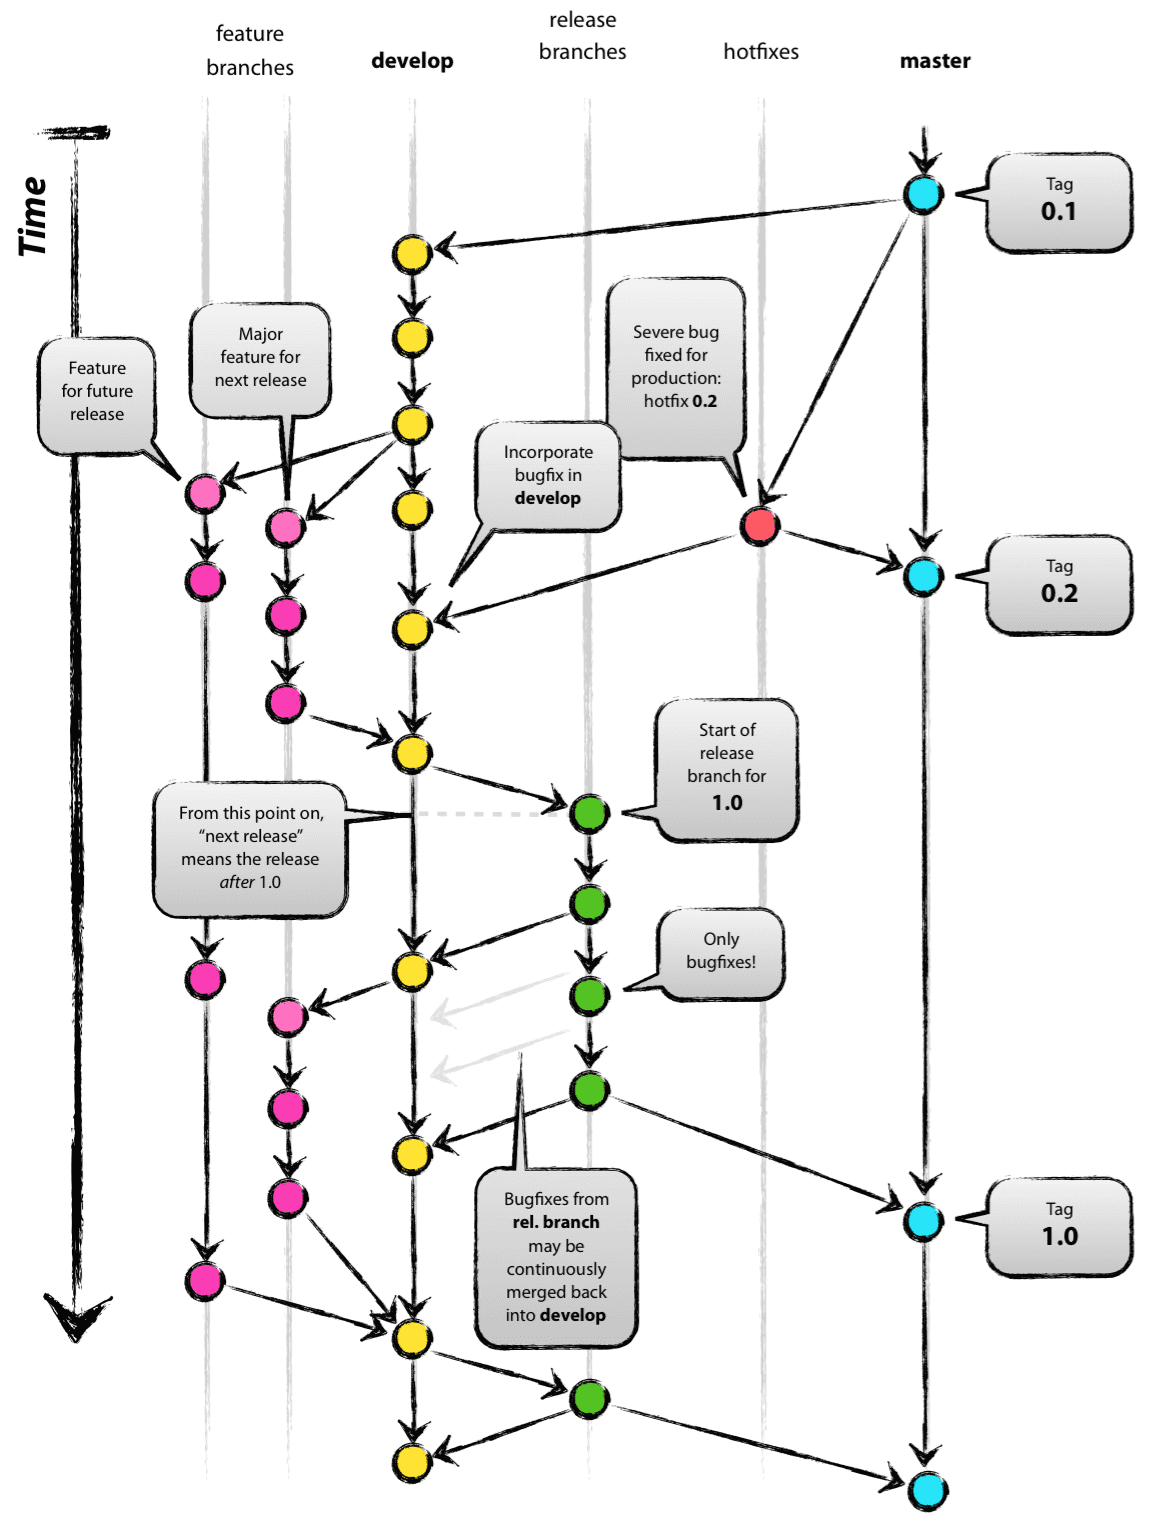
\includegraphics[scale=0.25]{gitflow.png}
		\caption{Styl pracy - Git Flow}
\end{figure}
\chapter{Eksperymenty} \label{ch:experiments}

\section{Parametry systemu testowego}

Testy przeprowadzane były na systemie
\begin{itemize}
	\item \textbf{OS}: Ubuntu 15.10,
    \item \textbf{Wersja kernela}: 4.2.0.16-generic,
    \item \textbf{Dysk}: Seagate ST1000DM003 1TB sATA III 64MB
    \begin{itemize}
    	\item \textbf{Format}: 3,5 cali,
        \item \textbf{Pojemność}: 1000 GB,
        \item \textbf{Interfejs}: Serial ATA III,
        \item \textbf{Prędkość obrotowa}: 7200 rpm,
        \item \textbf{Pamięć cache}: 64 MB,
        \item \textbf{Technologia przechowywania}: HDD,
        \item \textbf{Średnie opóźnienie}: 4,16 ms
    \end{itemize}
\end{itemize}
\section{Wyniki}

Poniżej przedstawiono otrzymane wyniki dla limitów szybkości transferu danych: 
\begin{itemize}
	\item bez limitów,
    \item 100 MB/s,
    \item 60 MB/s,
	\item 20 MB/s, 
    \item 5MB/s.
\end{itemize}

Dla każdej obliczono
\begin{itemize}
	\item przepustowość pasma,
    \item ilość operacji na sekundę,
    \item opóźnienie
\end{itemize}

\begin{figure}[h]
	\centering
	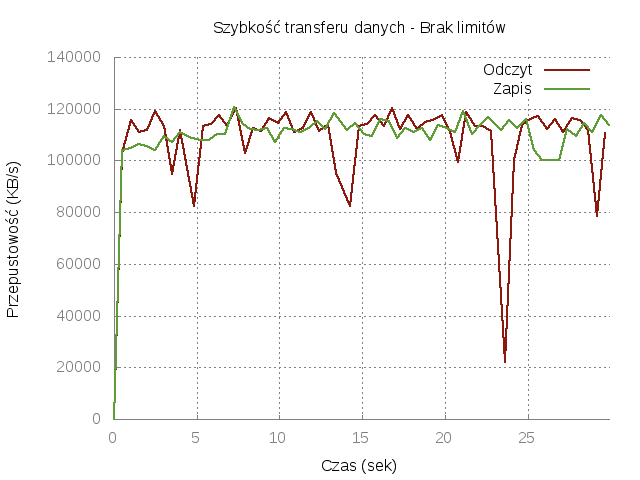
\includegraphics[scale=0.9]{results/Unlimited_bw.png}
		\caption{Brak limitów, przepustowość}
    \label{fig:unlimited-bw}
\end{figure}
\begin{figure}[h]
	\centering
	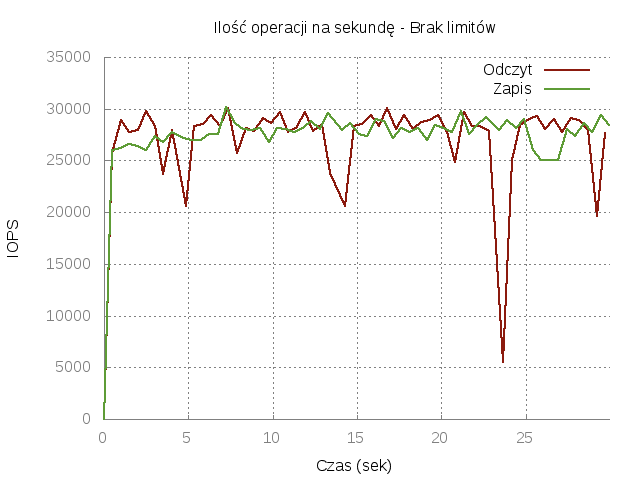
\includegraphics[scale=0.9]{results/Unlimited_iops.png}
		\caption{Brak limitów, ilość operacji na sekundę}
    \label{fig:unlimited-iops}
\end{figure}
\begin{figure}[h]
	\centering
	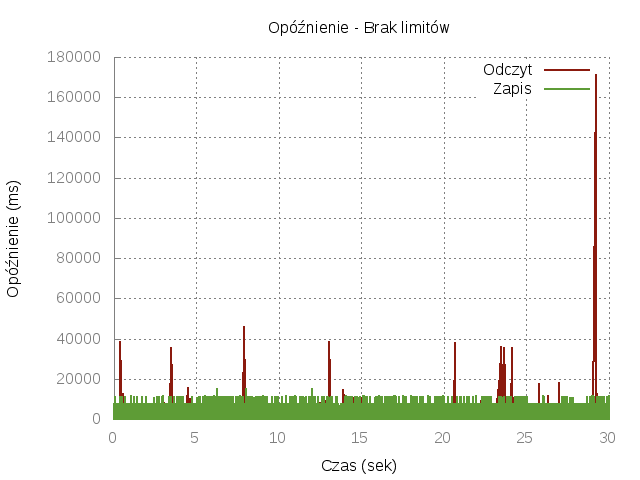
\includegraphics[scale=0.9]{results/Unlimited_lat.png}
		\caption{Brak limitów, opóźnienie}
    \label{fig:unlimited-lat}
\end{figure}

\begin{figure}[h]
	\centering
	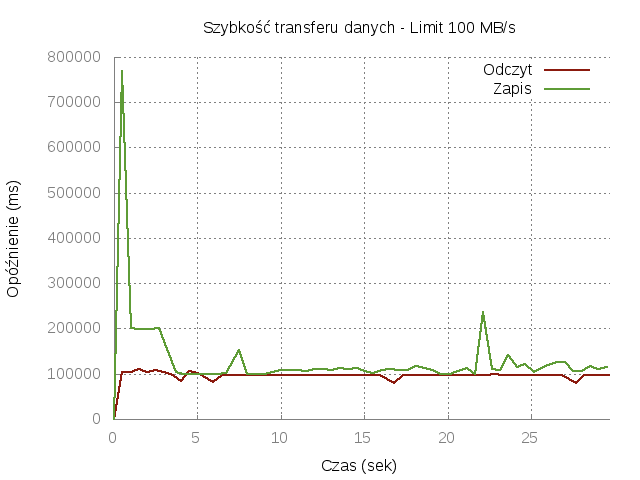
\includegraphics[scale=0.9]{results/100_bw.png}
		\caption{100 MB/s, przepustowość}
    \label{fig:100-bw}
\end{figure}
\begin{figure}[h]
	\centering
	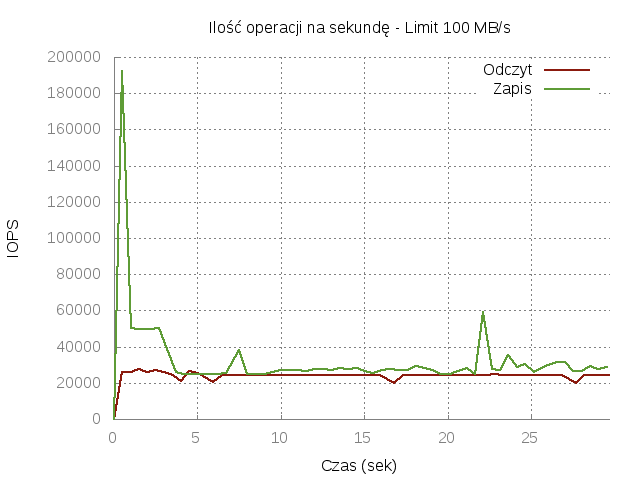
\includegraphics[scale=0.9]{results/100_iops.png}
		\caption{100 MB/s, ilość operacji na sekundę}
    \label{fig:100-iops}
\end{figure}
\begin{figure}[h]
	\centering
	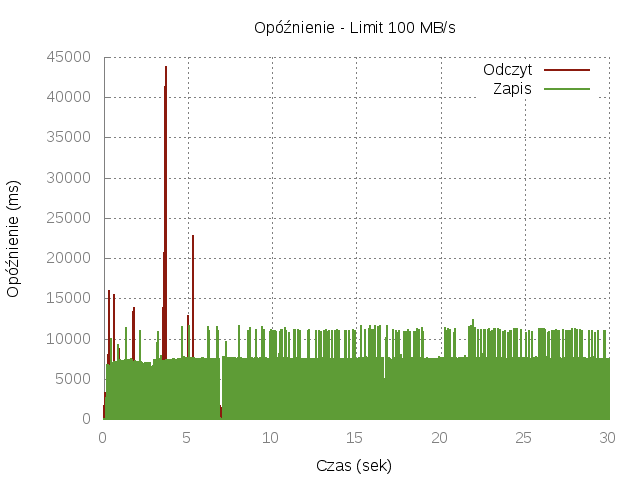
\includegraphics[scale=0.9]{results/100_lat.png}
		\caption{100 MB/s, opóźnienie}
    \label{fig:100-lat}
\end{figure}

\begin{figure}[h]
	\centering
	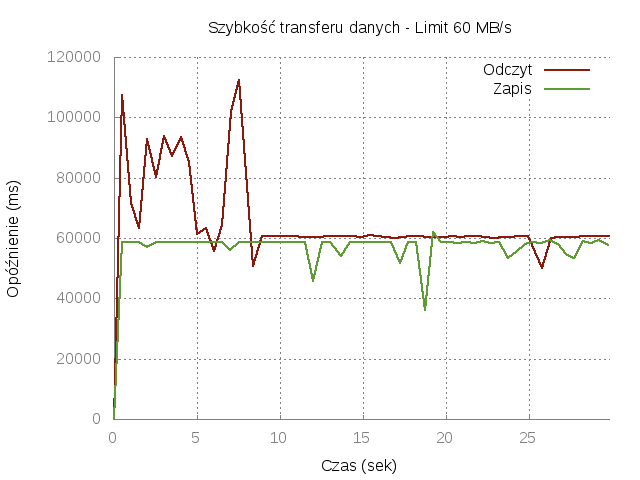
\includegraphics[scale=0.9]{results/60_bw.png}
		\caption{60 MB/s, przepustowość}
    \label{fig:60-bw}
\end{figure}
\begin{figure}[h]
	\centering
	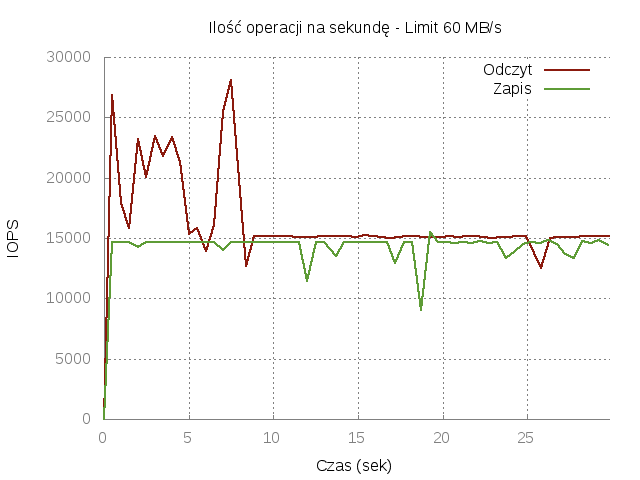
\includegraphics[scale=0.9]{results/60_iops.png}
		\caption{60 MB/s, ilość operacji na sekundę}
    \label{fig:60-iops}
\end{figure}
\begin{figure}[h]
	\centering
	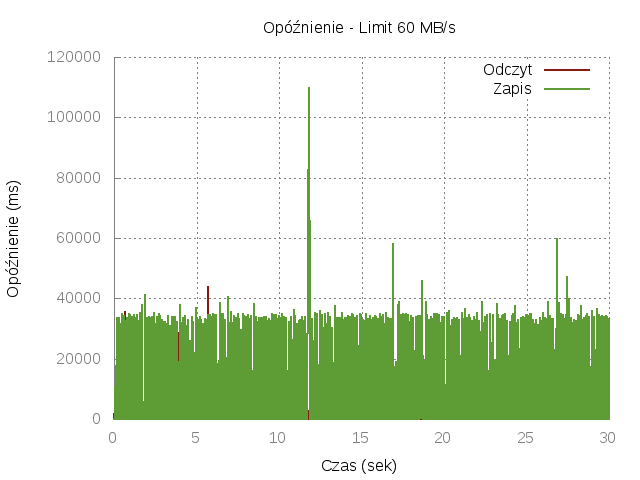
\includegraphics[scale=0.9]{results/60_lat.png}
		\caption{60 MB/s, opóźnienie}
    \label{fig:60-lat}
\end{figure}

\begin{figure}[h]
	\centering
	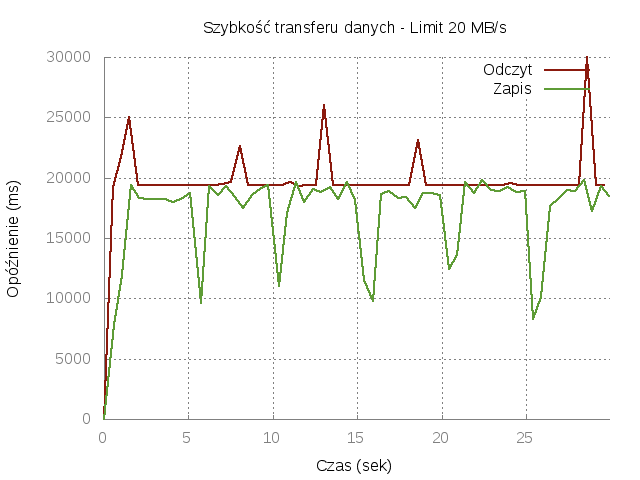
\includegraphics[scale=0.9]{results/20_bw.png}
		\caption{20 MB/s, przepustowość}
    \label{fig:20-bw}
\end{figure}
\begin{figure}[h]
	\centering
	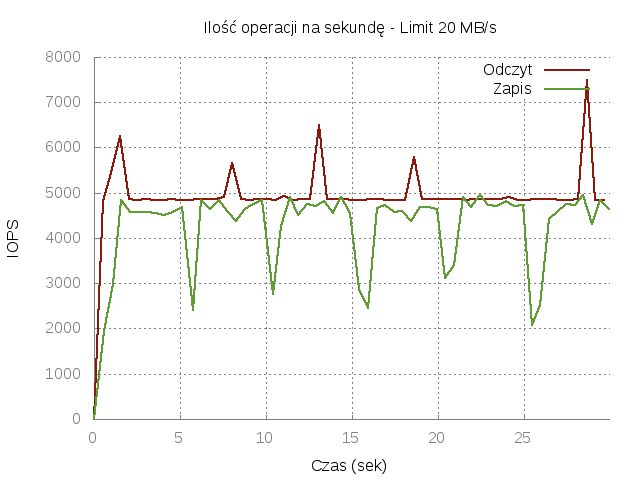
\includegraphics[scale=0.9]{results/20_iops.png}
		\caption{20 MB/s, ilość operacji na sekundę}
    \label{fig:20-iops}
\end{figure}
\begin{figure}[h]
	\centering
	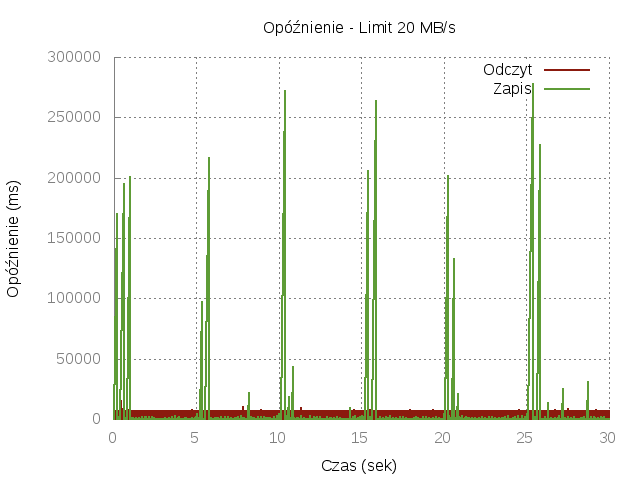
\includegraphics[scale=0.9]{results/20_lat.png}
		\caption{20 MB/s, opóźnienie}
    \label{fig:20-lat}
\end{figure}

\begin{figure}[h]
	\centering
	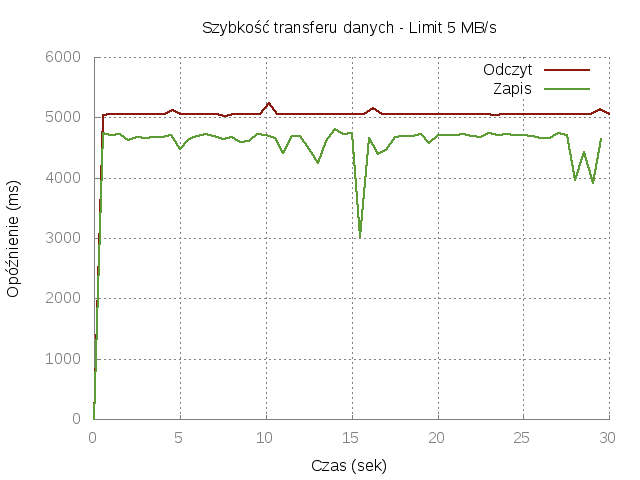
\includegraphics[scale=0.9]{results/5_bw.png}
		\caption{5 MB/s, przepustowość}
    \label{fig:5-bw}
\end{figure}
\begin{figure}[h]
	\centering
	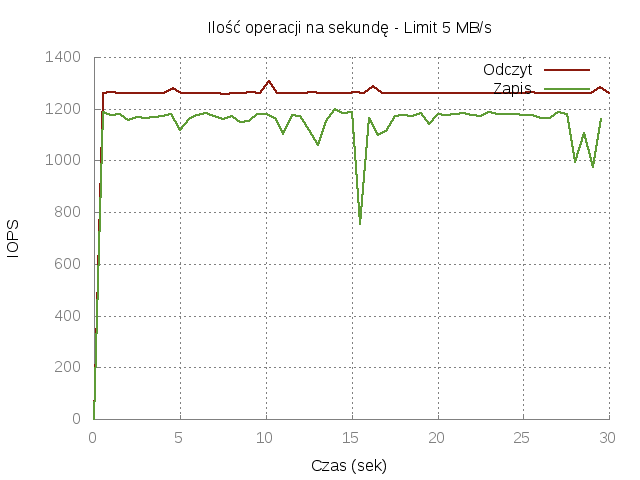
\includegraphics[scale=0.9]{results/5_iops.png}
		\caption{5 MB/s, ilość operacji na sekundę}
    \label{fig:5-iops}
\end{figure}
\begin{figure}[h]
	\centering
	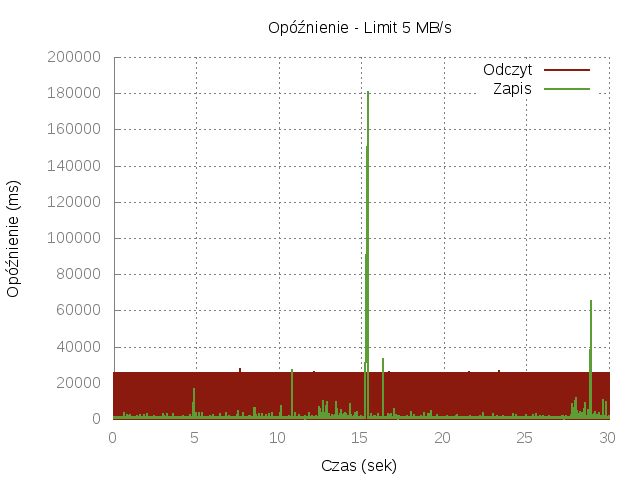
\includegraphics[scale=0.9]{results/5_lat.png}
		\caption{5 MB/s, opóźnienie}
    \label{fig:5-lat}
\end{figure}

\clearpage
\newpage
\section{Analiza wyników}
\subsection{Bez limitów}
Jak widać na wykresie \ref{fig:unlimited-bw}
nieograniczona szybkość transferu danych przyjmuje wartości z dużego zakresu. Dla operacji odczytu
waha się od \textbf{21933 Kb/s} do \textbf{120320 KB/s}, a dla zapisu od
\textbf{100000 KB/s} do \textbf{118400 KB/s}.

Ilość operacji na sekundę (IOPS, wykres \ref{fig:unlimited-iops}) jest powiązana bezpośrednio z szybkością transferu danych, dlatego
przebieg wykresu wygląda podobnie. Dla odczytu wartości wahają się
od \textbf{5483 IOPS} do \textbf{29696 IOPS}, a dla zapisu od \textbf{25000 IOPS}
do \textbf{29761 IOPS}.

Opóźnienie (wykres \ref{fig:unlimited-lat})
pokazują czas potrzebny na wykonanie operacji I/O. Wyraźnie widać, że
- dla odczytu - w okolicach 24 i 29 sekundy skoki w opóźnieniu opdowiadają
spadkom w szybkości transferu danych. Im dłuzszy czas potrzebny na przetworzenie
zlecenia operacji I/O, tym wolniejsza szybkość.

Na podstawie tych wyników można
zauważyć, że podczas przeprowadzania testów działają inne procesy, które
używają zasoby I/O, co powoduje spadki w szybkości transferu.

\subsection{100 MB/s}

Pierwszym z przeprowadzonych testów było ustawienie limitu szybkości zapisu i odczytu
na 100 Mb/s. Jak widać na wykresie \ref{fig:100-bw} i \ref{fig:100-iops}
podczas pierwszych 6 sekund
szybkość była niestabilna i przekroczyła narzucony limit dwukrotnie. Następnie, do końca testu,
utrzymywała się stabilnie poniżej 100 Mb/s a dwukrotnie spadła w okolice 80 Mb/s
(w 16 i 28 sekundzie). 

Początkową niestabilność można wytłumaczyć opóźnieniem (wykres \ref{fig:100-lat})
, które w pierwszych 6 sekundach miało niejednostajne wartości, różniące się nawet o
43 ms. Mimo tych nieregularności, szybkość transferu nigdy nie przekroczyła progu 111000 KB/s , co mieści się w 11\% narzuconego limitu. 

Dwa spadki w 16 i 28 sekundzie nie zależą od opóźnienia, a wywołane mogą być przez
chwilowy brak dostępnej szybkości. Jako, że nie przekraczają one limitu, nie stanowi to problemu
i system zadziałał prawidłowo.

Dla operacji zapisu szybkość transferu ustabilizowała sie wczesniej, koło 4 sekundy. Następnie utrzymywała się w okolicach limitu, poza dwoma momentami
(7 i 22 sekunda) gdzie wzrosła na chwilę nawet ponad 200 MB/s. Opóźnienia  utrzymywały się w okolicy 9 ms czasami zwiększając
się do 11ms.

\section{60 MB/s}

Dla odczytu limitowanego 60 MB/s szybkość stabilizowała się dłużej niż w przypadku 100 MB/s
- w okolicach 9 sekundy (wykres \ref{fig:60-bw} i \ref{fig:60-iops}).
Nastepnie wykorzystywana była przepustowość zgodna z założeniami, poza jednym spadkiem w
okolicach 26 sekundy. Stabilizacja szybkości jest również widoczna na wykresie \ref{fig:60-lat}, a spadek został spowodowany innymi czynnikami.

Wykres zapisu przebiega bardziej
chaotycznie. Od samego początku trzyma się ustalonych limitów, tylko raz osiągając
większą szybkość (odchył o 4\%) w 19 sekundzie. Wszystkie spadki spowodowane są opóźnieniem
dysku, co można zaobserwować na wykresie \ref{fig:60-lat}.

\section{20 MB/s}

Przy limicie ustawionym na 20 MB/s dla szybkości transferu danych podczas odczytu zaobserwowano największe odchyły od oczekiwanych wartości
(wykres \ref{fig:20-bw} i \ref{fig:20-iops}).
Przepustowość osiąga szybkości większe niż limit w okolicach 1, 7, 19, 29 sekundy.
Największy skok (w 29 sekundzie) osiąga 30 MB/s co stanowi 50\% limitu.

Skoki te są chwilowe i trwają krócej niż jedną sekundę a w pozostałych przypadkach
operacje są limitowane poprawnie. 

Opóźnienie (wykres \ref{fig:20-lat}) utrzymuje stałą wartość w okolicach 6 ms
z nielicznymi skokami do 8-10 ms oraz 14 ms na początku testu.

Wartości szybkości transferu danych, mimo iż nigdy nie przekroczyły limitu 20 MB/s  ciągle się
zmieniały. Zanotowano regularne spadki co około 5 sekund (6, 11, 16, 21, 26 sekunda)
w okolice 8200-10000 KB/s.

Spadki te łatwo wytłumaczyć obserwując opóźnienia (wykres \ref{fig:20-lat}).
Każdemu spadkowi odpowiada znaczny skok opóźnienia w okolice 200-260 ms.

\section{5 MB/s}

Dla najniższego z testowanych limitów - 5 MB/s szybkości transferu danych 
są najbardzie stabilne z wszystkich testowanych przypadków. Dla odczytu
(wykres \ref{fig:5-bw} i \ref{fig:5-iops}) w pierwszej sekundzie transfer osiąga szybkość w okolicach
5 MB/s i utrzymuje ją w całym czasie trwania testu z nieznacznymi skokami w
9, 10, 16 i 29 sekundzie. Skoki te nie przekraczają 5.3 MB/s, co stanowi 6\%
limitu.

Opóźnienie przyjmuje stała wartość 25 ms (wykres \ref{fig:5-lat}) z nielicznymi
małymi skokami.

Operacje zapisu również
nie przekraczają limitu 5 MB/s ale, tak samo jak w poprzednich przypadkach, pojawiają się spadki
szybkości transferu danych. Największy z nich ma miejsce w 16 sekundzie i osiąga wartość 3 MB/s.
Spadki te można zauważyć również badając opóźnienie (wykres \ref{fig:5-lat}).


\chapter{Podsumowanie i wnioski} \label{ch:summary}

\section{Wnioski}

Postawione cele zostały osiągnięte. Zaimplementowano system plików z mechanizmem
QoS, który pozwala na kontrolowanie wykorzystania przepustowości dla
operacji I/O. Pozwala on na ustalenie minimalnej szybkosci, która w miarę możliwości
nie zostaje przekroczona.

Pomimo skoków szybkości transferu danych ponad narzucony limit,
utrzymuje się ona w okolicach wyznaczonych wartości. Skoki te są
tylko chwilowe i niewielkie (najwyższy rzędu 11\% wartości limitu i 3,6\% przepustowości dysku, nie biorąc pod uwagę
skoków w 1 sekundzie) i nie zakłócają działania systemu.

Przeanalizowano system pod kątem szybkości transferu, ilości operacji na sekundę
oraz opóźnienia dysku. QoSFS działa, i może być przydatny w sytuacjach wymagających
stabilizacji szybkości transferu dla wybranych katalogów lub plików.

\section{Możliwości rozwoju}
Poniżej przedstawiono kilka przykładowych możliwości rozwoju projektu:
\ \\
\begin{enumerate}
	\item \textbf{Przechowywanie limitów szybkości transferu danych w inodach plików}. Dzięki takiemu zabiegowi możliwe będzie 
    nadanie osobnych limitów dla każdego pliku, a umieszczenie ich w inodach pozwoli na ich łatwe
     ustalanie z poziomu użytkownika. FUSE pozwala na tworzenie własnych implementacji
    inodów.
    
    \item \textbf{Zmienny deadline}. Deadline liczony dla każdego pliku w czasie wykonywania
    operacji I/O. Czas ten może zależeć np. od wielkości lub priorytetu pliku.
    
    \item \textbf{Dodatkowe schedulery}. Implementacja dodatkowych schedulerów biorących pod uwagę
    inne właściwości pliku, na którym wykonywana jest operacja.
    
    \item \textbf{Możliwośc ustalenia wykorzystywanej przepustowości}. Na chwilę obecną dostępna przepustowość
    liczona jest na podstawie różnicy pomiędzy maksymalną możliwą, a aktualnie używaną. 
    Nadanie tego limitu umożliwi używanie tylko części przepustowości
    dysku zapewniając zawsze dostępną minimalną szybkość transferu danych dla operacji na innych systemach plików.
    
    \item \textbf{Możliwośc przekroczenia ustalonej przepustowości}. Pozwolenie
    operacjom na przekroczenie narzuconej przepustowości w określonych
    warunkach jeżeli większa jest dostepna.
\end{enumerate}
\bibliographystyle{alpha}
\begin{thebibliography}{9}
\bibitem{bourbon}
Joel C. Wu, Scott A. Brandt\\
University of California, Santa Cruz\\
\emph{Providing Quality of Service Support in Object-Based File System}

\bibitem{apollon}
Taeseok Kim, Youjip Won, Doohan Kim, Kern Koh, and Yong H. Shin\\
School of Computer Science and Engineering, Seoul National University\\
Division of Electrical and Computer Engineering, Hanyang University\\
Dept. of Computer Science and Engineering, Seoul national Univeristy of Technology\\
\emph{Apollon: File System Level Support for QoS Augmented I/O}

\bibitem{virtualised}
Felipe Franciosi and William Knottenbelt\\
Departament of Computing, Imperial College London\\
\emph{Data Allocation Strategies for the Management of Quality of Service in Virtualised Storage Systems}

\bibitem{towards}
Felipe Franciosi and William Knottenbelt\\
\emph{Towards a QoS-aware Virtualised Storage System}

\bibitem{clouds}
Chien-Min Wang, Tse-Chen Yeh, Guo-Fu Tseng\\
Institute of Information Science, Academia Sinica, Taipei, Taiwan\\
\emph{Provision of Storage QoS in Distributed File Systems for Clouds}

\bibitem{zoran}
Zoran Dimitrijevic, Raju Rangaswami\\
\emph{Quality of Service Support for Real-time Storage Systems}

\bibitem{stevens}
W. Richard Stevens\\
\emph{Advanced Programming in the UNIX Environment (3rd edition)}

\bibitem{man}
Linux Manual\\
\emph{http://linux.die.net/man/}

\bibitem{vfs}
Dokumentacja VFS\\
\emph{http://tldp.org/LDP/tlk/fs/filesystem.html}

\bibitem{fuse}
Dokumentacja i przykłady FUSE\\
\emph{http://fuse.sourceforge.net/doxygen/index.html}

\bibitem{fio}
Dokumentacja fio\\
\emph{http://linux.die.net/man/1/fio}

\bibitem{cgroups}
Dokumentacja cgroups\\
\emph{http://www.kernel.org/doc/Documentation/cgroups/}
\end{thebibliography}
\nocite{*}

\end{document}
